% Left: Cayley table of the dihedral group D4 (rotations blue, reflections red). Right: the rotation axes of the cube. Generated by a short script.
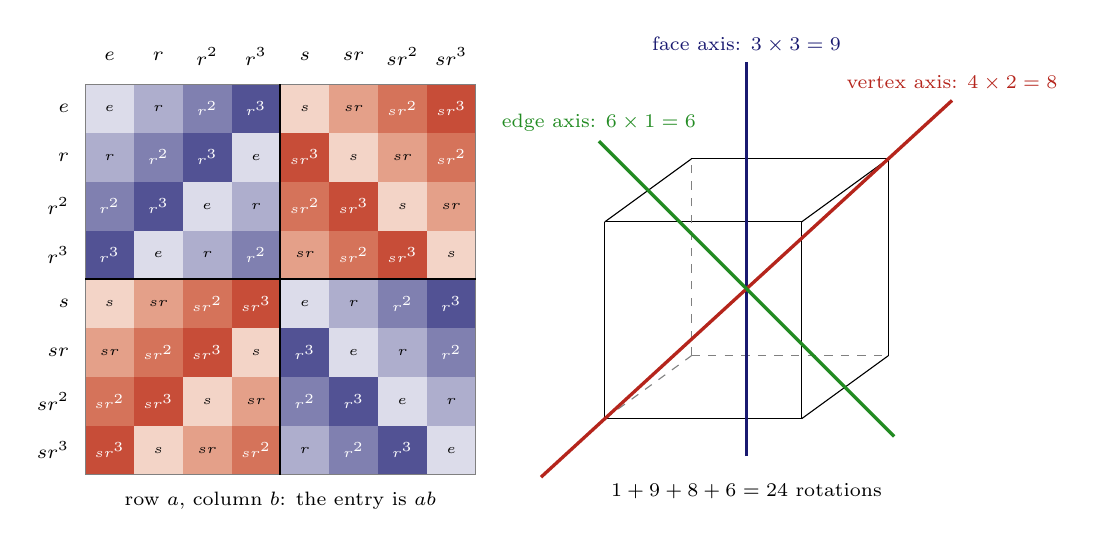
\begin{tikzpicture}
\begin{scope}
\node[font=\scriptsize] at (0.310,0.350) {$e$};
\node[font=\scriptsize,anchor=east] at (-0.080,-0.310) {$e$};
\node[font=\scriptsize] at (0.930,0.350) {$r$};
\node[font=\scriptsize,anchor=east] at (-0.080,-0.930) {$r$};
\node[font=\scriptsize] at (1.550,0.350) {$r^2$};
\node[font=\scriptsize,anchor=east] at (-0.080,-1.550) {$r^2$};
\node[font=\scriptsize] at (2.170,0.350) {$r^3$};
\node[font=\scriptsize,anchor=east] at (-0.080,-2.170) {$r^3$};
\node[font=\scriptsize] at (2.790,0.350) {$s$};
\node[font=\scriptsize,anchor=east] at (-0.080,-2.790) {$s$};
\node[font=\scriptsize] at (3.410,0.350) {$sr$};
\node[font=\scriptsize,anchor=east] at (-0.080,-3.410) {$sr$};
\node[font=\scriptsize] at (4.030,0.350) {$sr^2$};
\node[font=\scriptsize,anchor=east] at (-0.080,-4.030) {$sr^2$};
\node[font=\scriptsize] at (4.650,0.350) {$sr^3$};
\node[font=\scriptsize,anchor=east] at (-0.080,-4.650) {$sr^3$};
\fill[MidnightBlue!15] (0.000,0.000) rectangle (0.620,-0.620);
\node[font=\tiny,text=black] at (0.310,-0.310) {$e$};
\fill[MidnightBlue!35] (0.620,0.000) rectangle (1.240,-0.620);
\node[font=\tiny,text=black] at (0.930,-0.310) {$r$};
\fill[MidnightBlue!55] (1.240,0.000) rectangle (1.860,-0.620);
\node[font=\tiny,text=white] at (1.550,-0.310) {$r^2$};
\fill[MidnightBlue!75] (1.860,0.000) rectangle (2.480,-0.620);
\node[font=\tiny,text=white] at (2.170,-0.310) {$r^3$};
\fill[BrickRed!15] (2.480,0.000) rectangle (3.100,-0.620);
\node[font=\tiny,text=black] at (2.790,-0.310) {$s$};
\fill[BrickRed!35] (3.100,0.000) rectangle (3.720,-0.620);
\node[font=\tiny,text=black] at (3.410,-0.310) {$sr$};
\fill[BrickRed!55] (3.720,0.000) rectangle (4.340,-0.620);
\node[font=\tiny,text=white] at (4.030,-0.310) {$sr^2$};
\fill[BrickRed!75] (4.340,0.000) rectangle (4.960,-0.620);
\node[font=\tiny,text=white] at (4.650,-0.310) {$sr^3$};
\fill[MidnightBlue!35] (0.000,-0.620) rectangle (0.620,-1.240);
\node[font=\tiny,text=black] at (0.310,-0.930) {$r$};
\fill[MidnightBlue!55] (0.620,-0.620) rectangle (1.240,-1.240);
\node[font=\tiny,text=white] at (0.930,-0.930) {$r^2$};
\fill[MidnightBlue!75] (1.240,-0.620) rectangle (1.860,-1.240);
\node[font=\tiny,text=white] at (1.550,-0.930) {$r^3$};
\fill[MidnightBlue!15] (1.860,-0.620) rectangle (2.480,-1.240);
\node[font=\tiny,text=black] at (2.170,-0.930) {$e$};
\fill[BrickRed!75] (2.480,-0.620) rectangle (3.100,-1.240);
\node[font=\tiny,text=white] at (2.790,-0.930) {$sr^3$};
\fill[BrickRed!15] (3.100,-0.620) rectangle (3.720,-1.240);
\node[font=\tiny,text=black] at (3.410,-0.930) {$s$};
\fill[BrickRed!35] (3.720,-0.620) rectangle (4.340,-1.240);
\node[font=\tiny,text=black] at (4.030,-0.930) {$sr$};
\fill[BrickRed!55] (4.340,-0.620) rectangle (4.960,-1.240);
\node[font=\tiny,text=white] at (4.650,-0.930) {$sr^2$};
\fill[MidnightBlue!55] (0.000,-1.240) rectangle (0.620,-1.860);
\node[font=\tiny,text=white] at (0.310,-1.550) {$r^2$};
\fill[MidnightBlue!75] (0.620,-1.240) rectangle (1.240,-1.860);
\node[font=\tiny,text=white] at (0.930,-1.550) {$r^3$};
\fill[MidnightBlue!15] (1.240,-1.240) rectangle (1.860,-1.860);
\node[font=\tiny,text=black] at (1.550,-1.550) {$e$};
\fill[MidnightBlue!35] (1.860,-1.240) rectangle (2.480,-1.860);
\node[font=\tiny,text=black] at (2.170,-1.550) {$r$};
\fill[BrickRed!55] (2.480,-1.240) rectangle (3.100,-1.860);
\node[font=\tiny,text=white] at (2.790,-1.550) {$sr^2$};
\fill[BrickRed!75] (3.100,-1.240) rectangle (3.720,-1.860);
\node[font=\tiny,text=white] at (3.410,-1.550) {$sr^3$};
\fill[BrickRed!15] (3.720,-1.240) rectangle (4.340,-1.860);
\node[font=\tiny,text=black] at (4.030,-1.550) {$s$};
\fill[BrickRed!35] (4.340,-1.240) rectangle (4.960,-1.860);
\node[font=\tiny,text=black] at (4.650,-1.550) {$sr$};
\fill[MidnightBlue!75] (0.000,-1.860) rectangle (0.620,-2.480);
\node[font=\tiny,text=white] at (0.310,-2.170) {$r^3$};
\fill[MidnightBlue!15] (0.620,-1.860) rectangle (1.240,-2.480);
\node[font=\tiny,text=black] at (0.930,-2.170) {$e$};
\fill[MidnightBlue!35] (1.240,-1.860) rectangle (1.860,-2.480);
\node[font=\tiny,text=black] at (1.550,-2.170) {$r$};
\fill[MidnightBlue!55] (1.860,-1.860) rectangle (2.480,-2.480);
\node[font=\tiny,text=white] at (2.170,-2.170) {$r^2$};
\fill[BrickRed!35] (2.480,-1.860) rectangle (3.100,-2.480);
\node[font=\tiny,text=black] at (2.790,-2.170) {$sr$};
\fill[BrickRed!55] (3.100,-1.860) rectangle (3.720,-2.480);
\node[font=\tiny,text=white] at (3.410,-2.170) {$sr^2$};
\fill[BrickRed!75] (3.720,-1.860) rectangle (4.340,-2.480);
\node[font=\tiny,text=white] at (4.030,-2.170) {$sr^3$};
\fill[BrickRed!15] (4.340,-1.860) rectangle (4.960,-2.480);
\node[font=\tiny,text=black] at (4.650,-2.170) {$s$};
\fill[BrickRed!15] (0.000,-2.480) rectangle (0.620,-3.100);
\node[font=\tiny,text=black] at (0.310,-2.790) {$s$};
\fill[BrickRed!35] (0.620,-2.480) rectangle (1.240,-3.100);
\node[font=\tiny,text=black] at (0.930,-2.790) {$sr$};
\fill[BrickRed!55] (1.240,-2.480) rectangle (1.860,-3.100);
\node[font=\tiny,text=white] at (1.550,-2.790) {$sr^2$};
\fill[BrickRed!75] (1.860,-2.480) rectangle (2.480,-3.100);
\node[font=\tiny,text=white] at (2.170,-2.790) {$sr^3$};
\fill[MidnightBlue!15] (2.480,-2.480) rectangle (3.100,-3.100);
\node[font=\tiny,text=black] at (2.790,-2.790) {$e$};
\fill[MidnightBlue!35] (3.100,-2.480) rectangle (3.720,-3.100);
\node[font=\tiny,text=black] at (3.410,-2.790) {$r$};
\fill[MidnightBlue!55] (3.720,-2.480) rectangle (4.340,-3.100);
\node[font=\tiny,text=white] at (4.030,-2.790) {$r^2$};
\fill[MidnightBlue!75] (4.340,-2.480) rectangle (4.960,-3.100);
\node[font=\tiny,text=white] at (4.650,-2.790) {$r^3$};
\fill[BrickRed!35] (0.000,-3.100) rectangle (0.620,-3.720);
\node[font=\tiny,text=black] at (0.310,-3.410) {$sr$};
\fill[BrickRed!55] (0.620,-3.100) rectangle (1.240,-3.720);
\node[font=\tiny,text=white] at (0.930,-3.410) {$sr^2$};
\fill[BrickRed!75] (1.240,-3.100) rectangle (1.860,-3.720);
\node[font=\tiny,text=white] at (1.550,-3.410) {$sr^3$};
\fill[BrickRed!15] (1.860,-3.100) rectangle (2.480,-3.720);
\node[font=\tiny,text=black] at (2.170,-3.410) {$s$};
\fill[MidnightBlue!75] (2.480,-3.100) rectangle (3.100,-3.720);
\node[font=\tiny,text=white] at (2.790,-3.410) {$r^3$};
\fill[MidnightBlue!15] (3.100,-3.100) rectangle (3.720,-3.720);
\node[font=\tiny,text=black] at (3.410,-3.410) {$e$};
\fill[MidnightBlue!35] (3.720,-3.100) rectangle (4.340,-3.720);
\node[font=\tiny,text=black] at (4.030,-3.410) {$r$};
\fill[MidnightBlue!55] (4.340,-3.100) rectangle (4.960,-3.720);
\node[font=\tiny,text=white] at (4.650,-3.410) {$r^2$};
\fill[BrickRed!55] (0.000,-3.720) rectangle (0.620,-4.340);
\node[font=\tiny,text=white] at (0.310,-4.030) {$sr^2$};
\fill[BrickRed!75] (0.620,-3.720) rectangle (1.240,-4.340);
\node[font=\tiny,text=white] at (0.930,-4.030) {$sr^3$};
\fill[BrickRed!15] (1.240,-3.720) rectangle (1.860,-4.340);
\node[font=\tiny,text=black] at (1.550,-4.030) {$s$};
\fill[BrickRed!35] (1.860,-3.720) rectangle (2.480,-4.340);
\node[font=\tiny,text=black] at (2.170,-4.030) {$sr$};
\fill[MidnightBlue!55] (2.480,-3.720) rectangle (3.100,-4.340);
\node[font=\tiny,text=white] at (2.790,-4.030) {$r^2$};
\fill[MidnightBlue!75] (3.100,-3.720) rectangle (3.720,-4.340);
\node[font=\tiny,text=white] at (3.410,-4.030) {$r^3$};
\fill[MidnightBlue!15] (3.720,-3.720) rectangle (4.340,-4.340);
\node[font=\tiny,text=black] at (4.030,-4.030) {$e$};
\fill[MidnightBlue!35] (4.340,-3.720) rectangle (4.960,-4.340);
\node[font=\tiny,text=black] at (4.650,-4.030) {$r$};
\fill[BrickRed!75] (0.000,-4.340) rectangle (0.620,-4.960);
\node[font=\tiny,text=white] at (0.310,-4.650) {$sr^3$};
\fill[BrickRed!15] (0.620,-4.340) rectangle (1.240,-4.960);
\node[font=\tiny,text=black] at (0.930,-4.650) {$s$};
\fill[BrickRed!35] (1.240,-4.340) rectangle (1.860,-4.960);
\node[font=\tiny,text=black] at (1.550,-4.650) {$sr$};
\fill[BrickRed!55] (1.860,-4.340) rectangle (2.480,-4.960);
\node[font=\tiny,text=white] at (2.170,-4.650) {$sr^2$};
\fill[MidnightBlue!35] (2.480,-4.340) rectangle (3.100,-4.960);
\node[font=\tiny,text=black] at (2.790,-4.650) {$r$};
\fill[MidnightBlue!55] (3.100,-4.340) rectangle (3.720,-4.960);
\node[font=\tiny,text=white] at (3.410,-4.650) {$r^2$};
\fill[MidnightBlue!75] (3.720,-4.340) rectangle (4.340,-4.960);
\node[font=\tiny,text=white] at (4.030,-4.650) {$r^3$};
\fill[MidnightBlue!15] (4.340,-4.340) rectangle (4.960,-4.960);
\node[font=\tiny,text=black] at (4.650,-4.650) {$e$};
\draw[gray,thin] (0,0) rectangle (4.960,-4.960);
\draw[black,thick] (2.480,0) -- (2.480,-4.960) (0,-2.480) -- (4.960,-2.480);
\node[font=\scriptsize,anchor=north] at (2.480,-5.060) {row $a$, column $b$: the entry is $ab$};
\end{scope}
\begin{scope}
\draw[black] (6.600,-4.250) -- (6.600,-1.750);
\draw[gray,dashed] (6.600,-4.250) -- (7.700,-3.450);
\draw[black] (6.600,-4.250) -- (9.100,-4.250);
\draw[black] (6.600,-1.750) -- (7.700,-0.950);
\draw[black] (6.600,-1.750) -- (9.100,-1.750);
\draw[gray,dashed] (7.700,-3.450) -- (7.700,-0.950);
\draw[gray,dashed] (7.700,-3.450) -- (10.200,-3.450);
\draw[black] (7.700,-0.950) -- (10.200,-0.950);
\draw[black] (9.100,-4.250) -- (9.100,-1.750);
\draw[black] (9.100,-4.250) -- (10.200,-3.450);
\draw[black] (9.100,-1.750) -- (10.200,-0.950);
\draw[black] (10.200,-3.450) -- (10.200,-0.950);
\draw[MidnightBlue,very thick] (8.400,-4.725) -- (8.400,0.275);
\node[MidnightBlue,font=\scriptsize,anchor=south,align=left] at (8.400,0.275) {face axis: $3\times3=9$};
\draw[BrickRed,very thick] (5.790,-4.992) -- (11.010,-0.208);
\node[BrickRed,font=\scriptsize,anchor=south,align=left] at (11.010,-0.208) {vertex axis: $4\times2=8$};
\draw[ForestGreen,very thick] (10.275,-4.475) -- (6.525,-0.725);
\node[ForestGreen,font=\scriptsize,anchor=south,align=left] at (6.525,-0.725) {edge axis: $6\times1=6$};
\node[font=\scriptsize,anchor=north] at (8.4,-4.95) {$1+9+8+6=24$ rotations};
\end{scope}
\end{tikzpicture}
